% COSA.tex
\documentclass{beamer}
\usepackage{amsmath,amsthm, amsfonts, amssymb, amsxtra,amsopn,epsfig,float}
\usepackage[lined,boxed,commentsnumbered]{algorithm2e}
\usepackage{listings}
\usetheme{default}

\title[Parallel COSA]{A short talk on parallelizing COSA}
%\subtitle[Errors]{Plus a self introduction}
\author[Jiading Gai]{Jiading Gai}
\institute[ND]{
  Center for Research Computing\\
  University of Notre Dame\\
  Notre Dame, IN 46556\\[1ex]
  \texttt{jgai@nd.edu}
}
\date[Aug 2010]{Aug 23, 2010}


\begin{document}
\maketitle
% \begin{frame}
% \frametitle{Self Introduction}
% \begin{figure}
%  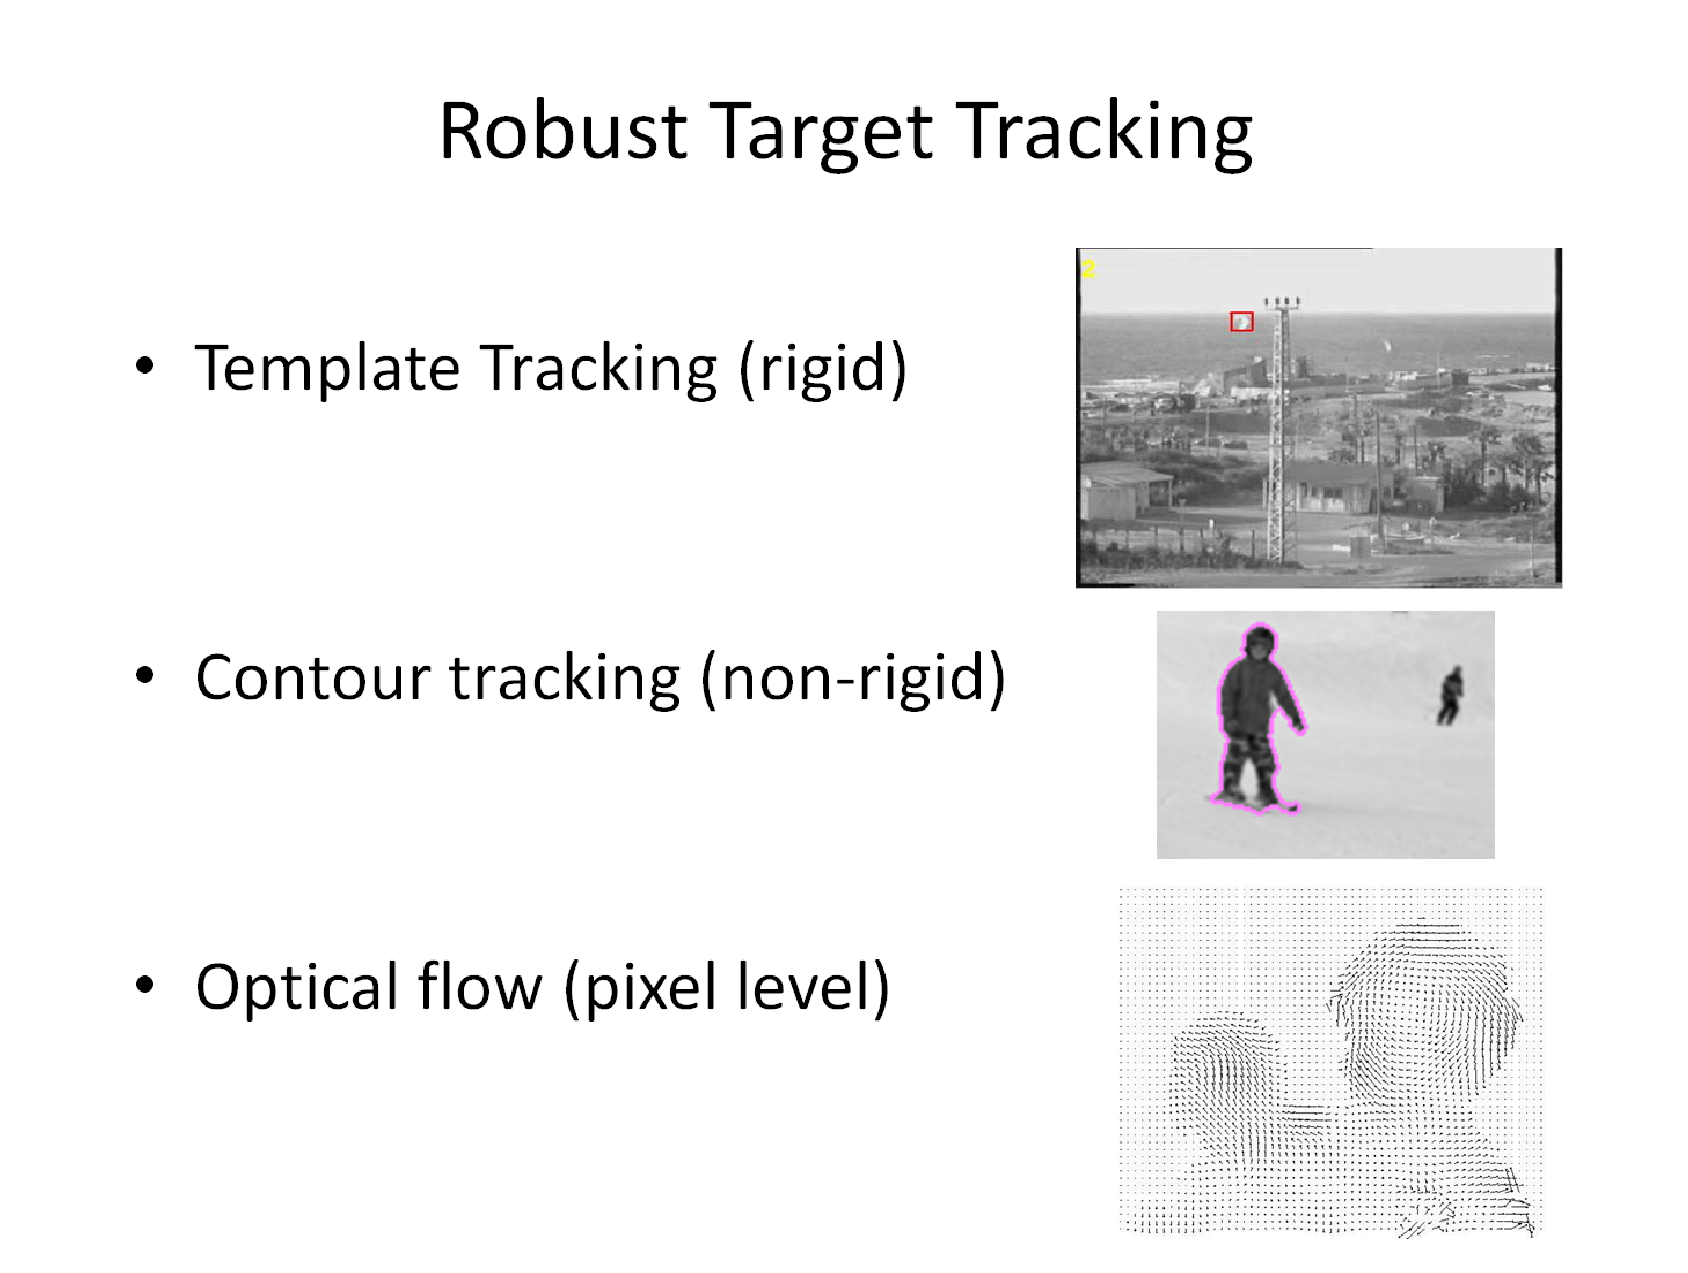
\includegraphics[width=\textwidth]{figures/a.eps}
% \end{figure}
% \end{frame}

% \begin{frame}
%   \frametitle{Introduction}

% N objects $\to$ L clusters:
% \[
% c(i)=l \Rightarrow i \in G_l~(1\leq i \leq N, 1 \leq l \leq L)
% \]

% Classic cluster analysis (minimizing):

% \[
% Q(c)=\sum^{L}_{l=1}\frac{W_l}{N^2_l}\sum_{c(i)=l}\sum_{c(j)=l}D_{ij}
% \]

% \begin{itemize}
% \item Each object $i$ has $n$ attributes:$x_i=(x_{i1},...,x_{in})$
% \item $D_{ij}=\sum^n_{k=1}w_kd_{ijk}$, 

% where $d_{ijk}=\frac{|x_{ik}-x_{jk}|}{s_k}$; $s_k=\frac{1}{N^2}\sum^N_{i=1}\sum^N_{j=1}|x_{ik}-x_{jk}|$.
% \end{itemize}
% \end{frame}


% \begin{frame}
% \frametitle{Feature Selection}
% Clustering on a fixed subset of the attributes (jointly minimizing):

% \[
% Q(c,\textbf{w})=\sum^{L}_{l=1}\frac{W_l}{N^2_l}\sum_{c(i)=l}\sum_{c(j)=l}D_{ij}[\textbf{w}]
% \]
% \begin{itemize}
% \item $\textbf{w}=\{w_k\}^n_1$.
% \item $D_{ij}[\textbf{w}]=\sum^n_{k=1}w_kd_{ijk}$.
% \end{itemize}
% \end{frame}

\begin{frame}
\frametitle{Clustering on different subsets of the attributes (COSA):}
N objects $\to$ L clusters:
\[
c(i)=l \Rightarrow i \in G_l~(1\leq i \leq N, 1 \leq l \leq L)
\]

\[
Q(c,\{\textbf{w}_l\}^{L}_1)=\sum^{L}_{l=1}\frac{W_l}{N^2_l}\sum_{c(i)=l}\sum_{c(j)=l}D_{ij}[\textbf{w}_l]
\]
\begin{itemize}
\item Each object $i$ has $n$ attributes:$x_i=(x_{i1},...,x_{in})$
\item $\textbf{w}_l=\{w_{kl}\}^n_1$, $1 \leq l \leq L$.
\item $D_{ij}[\textbf{w}_l]=\sum^n_{k=1}w_{kl}d_{ijk}$,
where $d_{ijk}=\frac{|x_{ik}-x_{jk}|}{s_k}$; $s_k=\frac{1}{N^2}\sum^N_{i=1}\sum^N_{j=1}|x_{ik}-x_{jk}|$.
\item Augumented to avoid clustering only on a single attribute:

$D_{ij}[\textbf{w}_l]~~\rightarrow~~D^{(\lambda)}_{ij}[\textbf{w}_l]$.
\end{itemize}
\end{frame}

\begin{frame}
\frametitle{Minimization Scheme}
%Applying an alternating optimization strategy on

% \[
% Q(c,\{\textbf{w}_l\}^{L}_1)=\sum^{L}_{l=1}\frac{W_l}{N^2_l}\sum_{c(i)=l}\sum_{c(j)=l}D^{\lambda}_{ij}[\textbf{w}_l]
% \]

\begin{itemize}
\item Start with an initial guess for $w_{ki}=\frac{1}{n}$, $\eta=\lambda$
\item \textbf{outer WHILE}
     \item \textbf{inner WHILE}
\item Fix $w_{ki}$, minimize the criterion w.r.t the encoder $c(\cdot)$
  \begin{itemize}
  \item $D^{(\eta)}_{ij}[\textbf{w}]=-\eta \cdot \log \sum^{n}_{k=1}w_{ki} \cdot e^{-\frac{d_{ijk}}{\eta}}$.
  $d_{ijk}=\frac{|x_{ik}-x_{jk}|}{s_k}$,~~$s_k=\frac{1}{N^2}\sum^N_{i=1}\sum^N_{j=1}|x_{ik}-x_{jk}|$.
  \item $D^{1}_{ij}[\textbf{W}]=\max(D^{(\eta)}_{ij}[\textbf{w}_{c(i|\textbf{W})}],D^{(\eta)}_{ij}[\textbf{w}_{c(j|\textbf{W})}])$ (30) \\
        $D_{ij}^{(2)}[\textbf{W}]=\sum^n_{k=1}\max(w_{k,c(i|\textbf{W})},w_{k,c(j|\textbf{W})})d_{ijk}$ (33)
  \item KNN$(i)=\{j|D_{ij} \leq d_{i(K)}\}$.
  \end{itemize}
\item Fix $c(\cdot)$, minimize the criterion w.r.t the weights $w_{ki}$
  \begin{itemize}
    \item $w_{ki}=\frac{e^{-\frac{S_{ki}}{\lambda}}}{\sum^n_{k'=1}e^{-\frac{S_{ki}}{\lambda}}}$, $S_{ki}=\frac{1}{K}\sum_{j \in KNN(i)}d_{ijk}$.
  \end{itemize}
\item \textbf{END inner WHILE}
\item Increment $\eta=\eta+\alpha \cdot \lambda$
\item \textbf{END outer WHILE}
\item This iterative procedure is continued until convergence.
\end{itemize}
\end{frame}

\begin{frame}
Parallel COSA algorithm:
\begin{center} 
  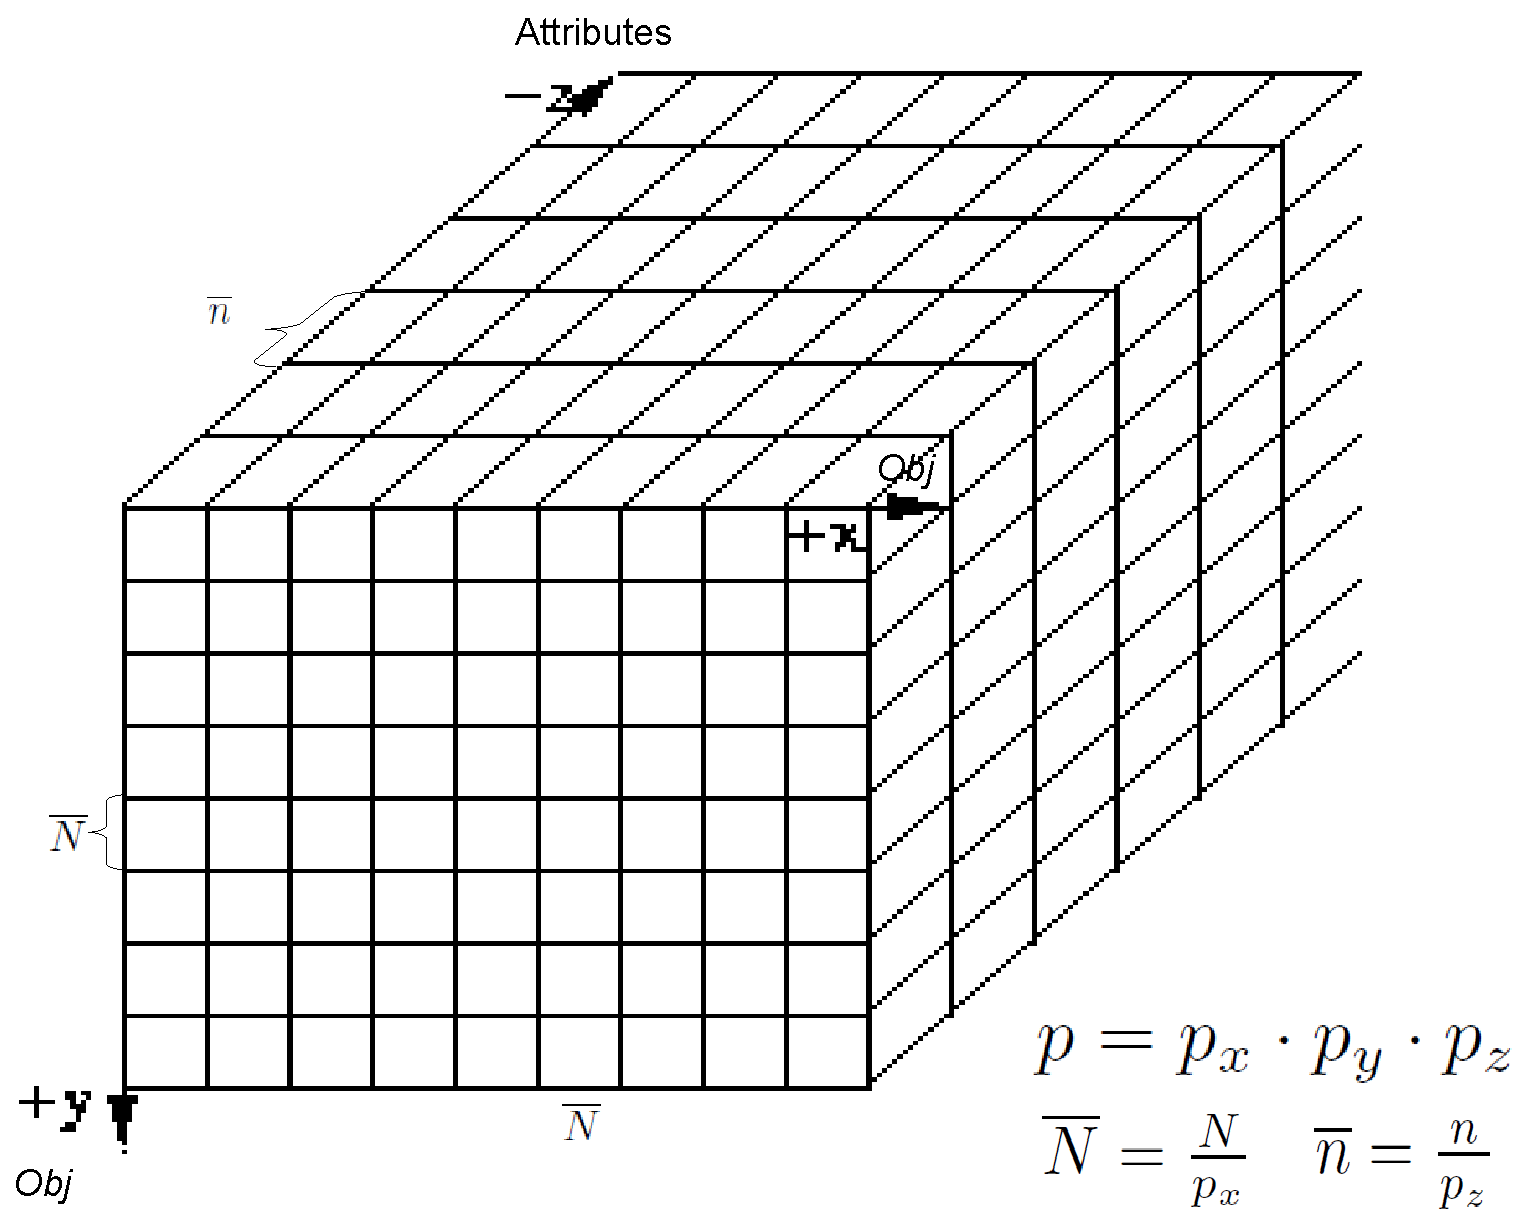
\includegraphics[width=0.8\textwidth]{figures/3d_data.eps} 
\end{center}
\end{frame}



\begin{frame}
\frametitle{Observed speedup on a real-world data}
c22\_ceu.txt: (N=1000, n=13,000) \\
DELL R810 with 24 Xeon processors and a total 132GB memory
\begin{center}
    \begin{tabular}{ | l | l | l | l | l |}
    \hline
      p   & $p_x$ & $p_y$   &  $p_z$  & time\\ \hline
      1   & 1     & 1          & 1      & 105417.38615 sec\\ \hline
      2   & 1     & 1          & 2      & 51324.306341 sec\\ \hline
      3   & 1     & 1          & 3      & 33812.867425 sec\\ \hline
      4   & 1     & 1          & 4      & 26374.128593 sec\\ \hline
      5   & 1     & 1          & 5      & 20340.902349 sec\\ \hline
      6   & 1     & 1          & 6      & 17151.958595 sec\\ \hline
      8   & 2     & 2          & 2      & 12327.523793 sec\\ \hline
      12  & 2     & 2          & 3      & 9007.370069  sec\\ \hline
      16  & 2     & 2          & 4      & 6559.531571  sec\\ \hline
      20  & 2     & 2          & 5      & 5273.171368  sec\\ \hline
      24  & 2     & 2          & 6      & 4778.485166  sec\\ \hline
    \end{tabular}
\end{center}
\end{frame}

\begin{frame}
\begin{center} 
  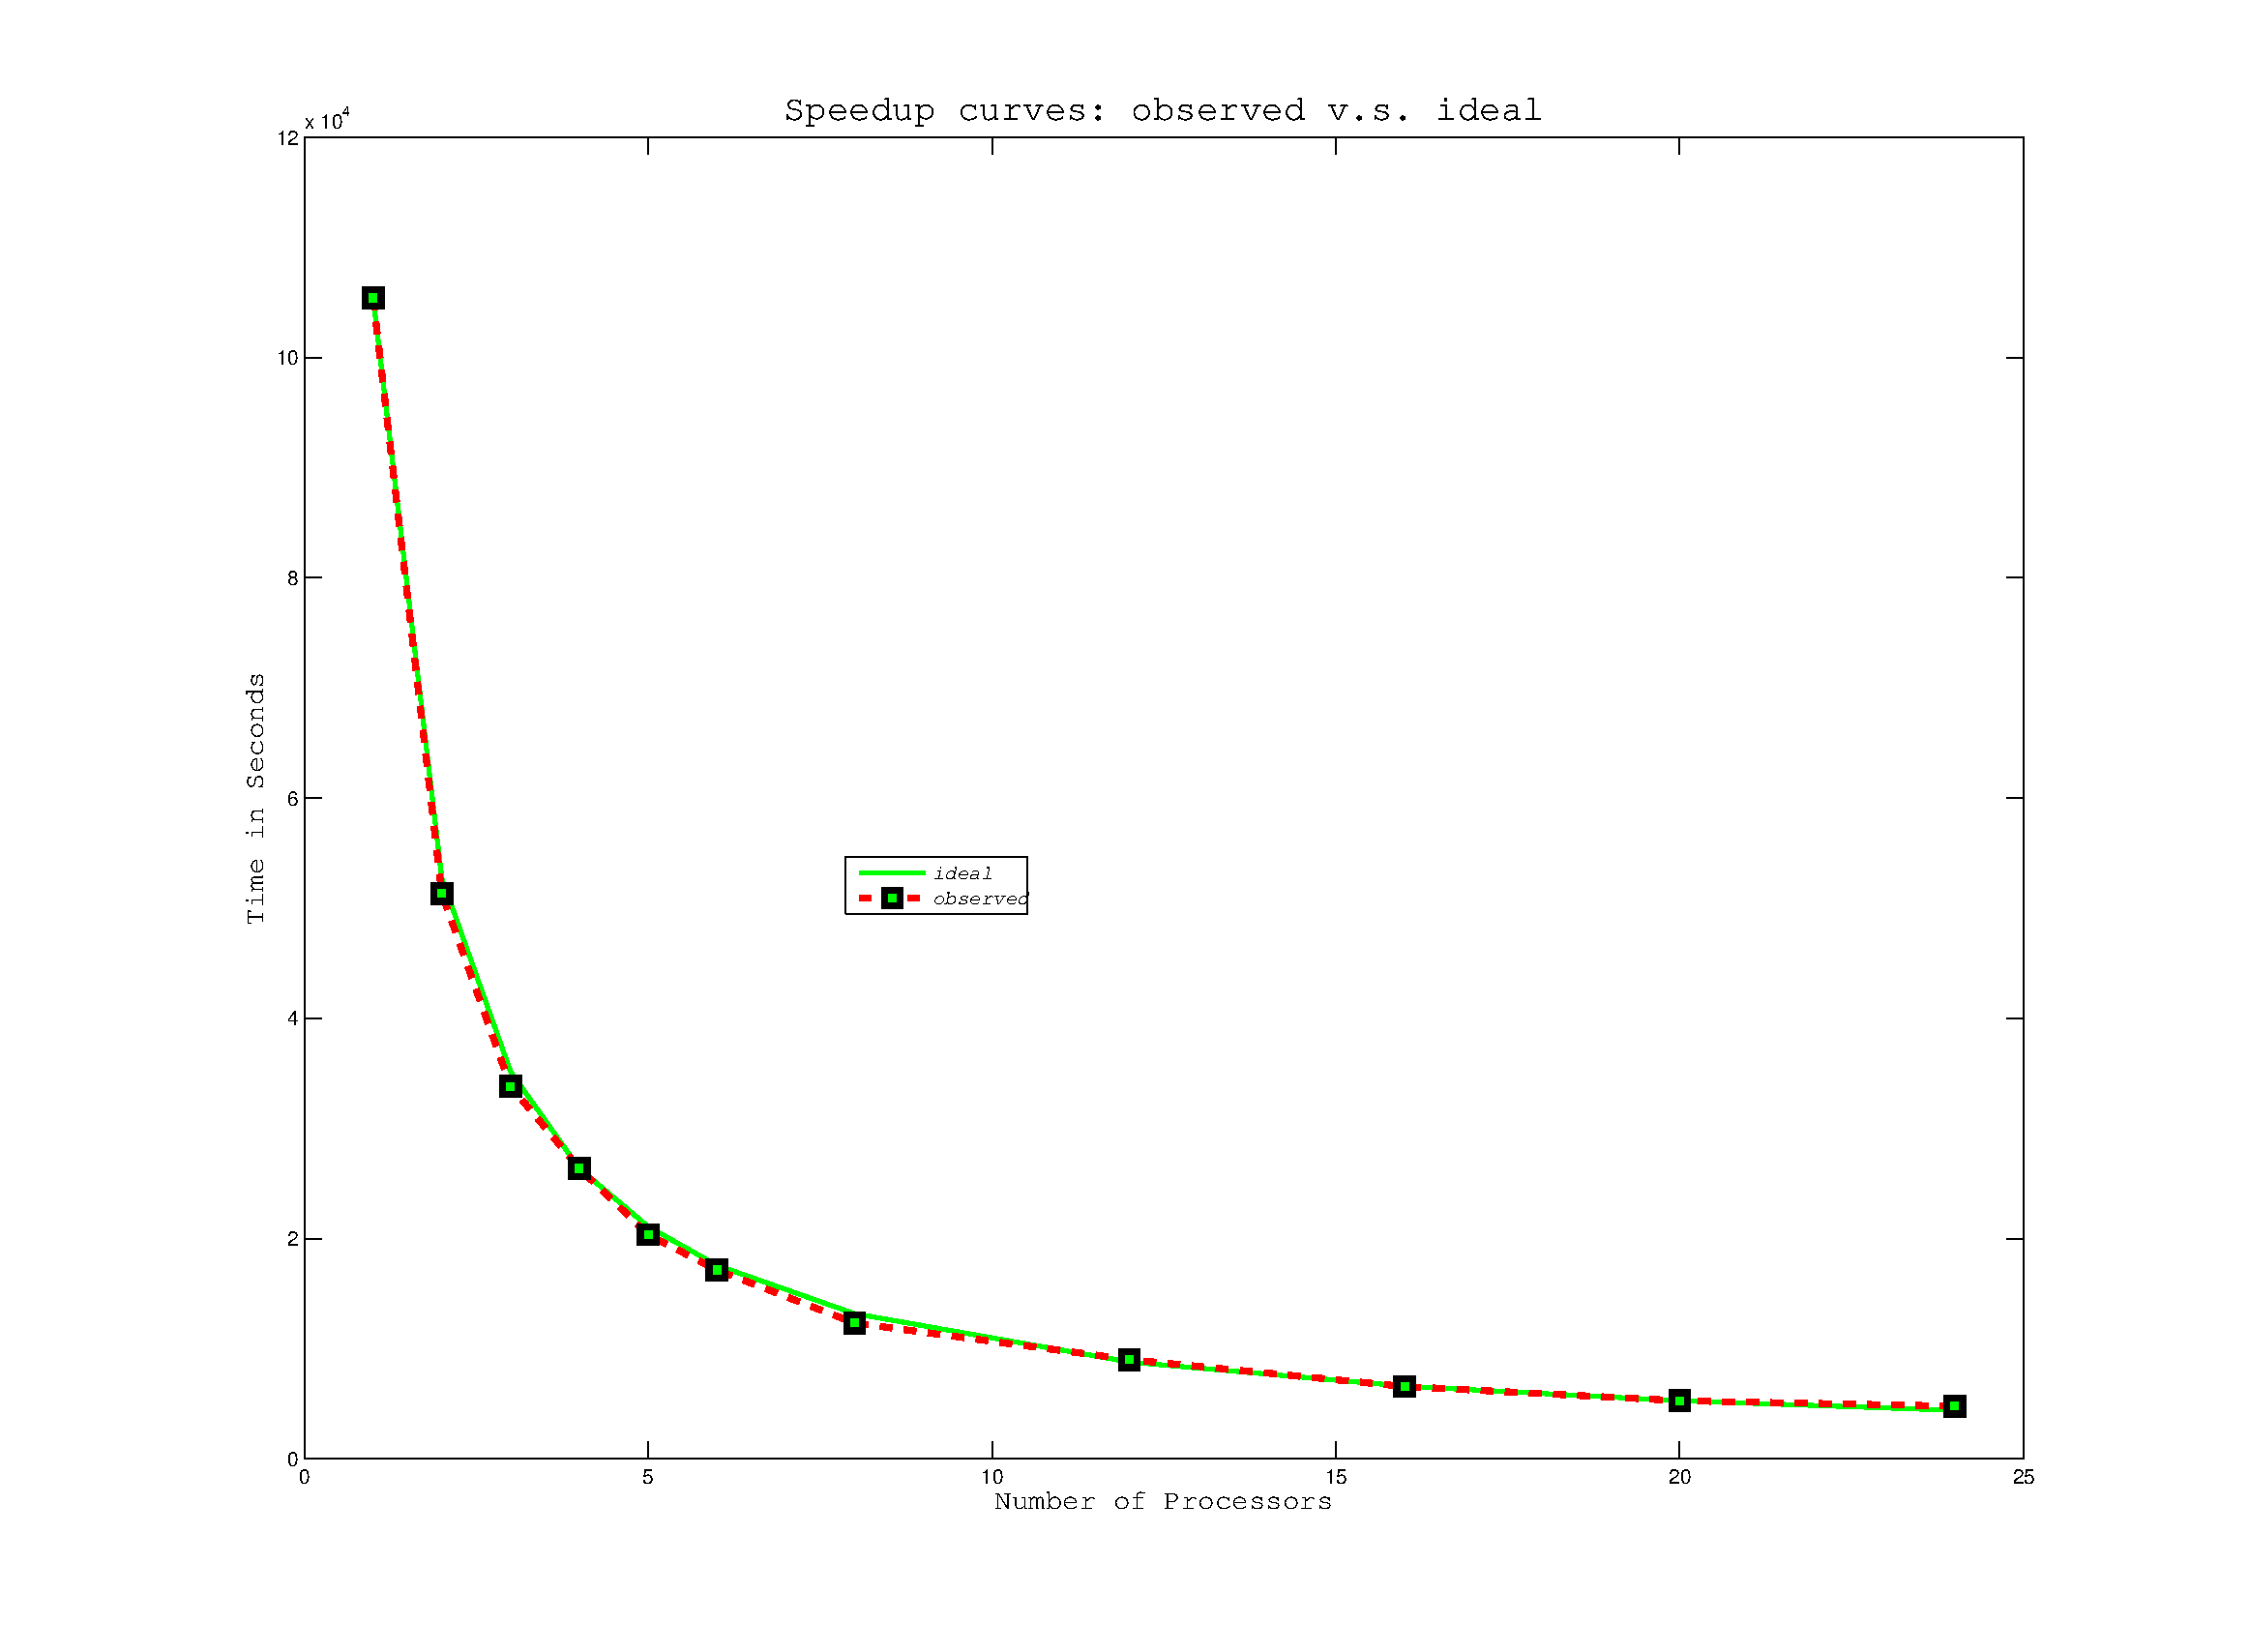
\includegraphics[width=1.0\textwidth]{figures/speedup.eps} 
\end{center}
\end{frame}

\begin{frame}
\frametitle{Conclusion}
\begin{itemize}
\item Matching performance between MPI-COSA and Fortran-COSA executable (released by the original authors)
\item MPI-COSA Source code was released publicly on launchpad.net
\end{itemize}
\begin{center} 
  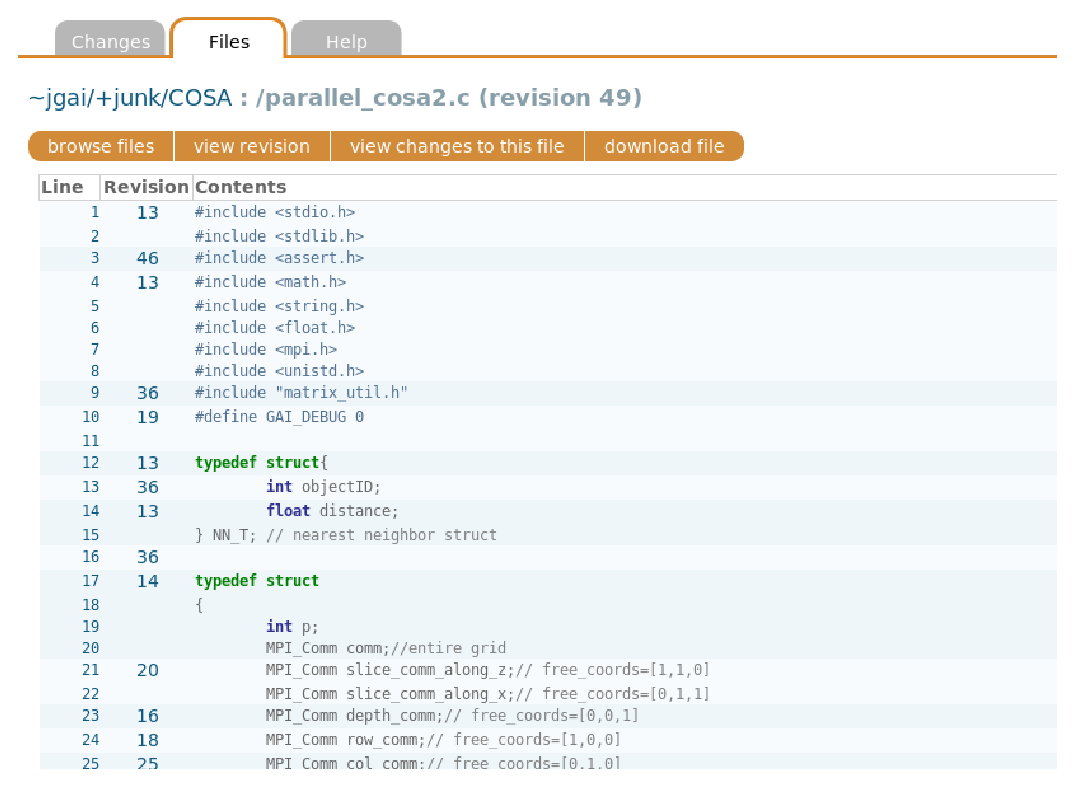
\includegraphics[height=0.5\textwidth]{figures/mybzr2.eps} 
\end{center}
\end{frame}

\begin{frame}
\frametitle{Performance Analysis}
Sequential COSA:
\begin{eqnarray}
T_1&=&[4N^2+(10n+2K)N^2+(5K+5)nN+3n+N] \cdot T^{flop} \cdot \mathbb{T} \nonumber 
\end{eqnarray}
Parallel COSA :\\
($p=p_x \cdot p_y \cdot p_z$, $\overline{N}=\frac{N}{p_x}$, $\overline{n}=\frac{n}{p_z}$)
\begin{eqnarray}
T^{comp}_q&=& [5\overline{N}^2+(10\overline{n}+2K)\overline{N}^2+(5K+5)\overline{n}\overline{N}+\nonumber \\ &&(2K+1)\overline{N}\cdot p_x \cdot K+2\overline{N}+2\overline{n}] \cdot T^{flop} \cdot \mathbb{T}\nonumber \\
T^{comm}_q&=& [\overline{n}\cdot p_x p_y \cdot \log(p_xp_y)+\overline{N}^2\cdot p_z \log(p_z)+2\overline{N}^2+\nonumber \\ &&3\overline{N}K\cdot p_x \log(p_x)+\overline{n}\overline{N}\cdot p_x\log(p_x)+\overline{N}\cdot p_z \log(p_z)+\nonumber \\ &&p\log(p)] \cdot T^{Transmit} \cdot \mathbb{T}\nonumber
\end{eqnarray}
\begin{eqnarray}
T_q&=&T^{comp}_q+T^{comm}_q \nonumber \\
&=&[\frac{6N^2n}{q}+\frac{N^2}{q}+\frac{N^2}{q}\log(\frac{N}{p})+pK+\frac{nNK}{p}+\frac{n^2N}{p}+\frac{2nN}{p}] \cdot\nonumber \\
&& T^{flop} \cdot \mathbb{T}+[np\log(p)+2pK] \cdot T^{Transmit} \cdot \mathbb{T} \nonumber
\end{eqnarray}
\end{frame}

\begin{frame}
\frametitle{Performance Analysis:}
\begin{eqnarray}
T_q&=&T^{comp}_q+T^{comm}_q \nonumber \\
&=&[\frac{6N^2n}{q}+\frac{N^2}{q}+\frac{N^2}{q}\log(\frac{N}{p})+pK+\frac{nNK}{p}+\frac{n^2N}{p}+\frac{2nN}{p}] \cdot\nonumber \\
&& T^{flop} \cdot \mathbb{T}+[np\log(p)+2pK] \cdot T^{Transmit} \cdot \mathbb{T} \nonumber
\end{eqnarray}

\begin{itemize}
\item $T^{Transmit}$ is the time of sending a single message containing a floating point number.
\item $T^{comm}_q$ is insignificant compared to $T^{comp}_q$, as $N$ increases.
For example
\begin{itemize}
\item $N=11,000$, $n=2,000$, $K=\sqrt{N}=105$ and $q=16 (p=4)$
\item $T^{Transmit}=10 \times 10^{-6}~seconds$, $T^{flop}=7 \times 10^{-11}~seconds$
$T^{comp}_q= 5.9875 \cdot \mathbb{T} \gg T^{comm}_q= 0.1684 \cdot \mathbb{T}$
\end{itemize}
\end{itemize}
Predicted Speedup:
\begin{eqnarray}
S=\frac{T_1}{T_q}=\frac{[6N^2n+N^2+N\log(N)+KnN+n^2N+2nN] \cdot T^{flop} \cdot \mathbb{T}}{T^{comp}_q+T^{comm}_q} \nonumber
\end{eqnarray}
\end{frame}

\end{document}
%%%%%%%%%%%%%%%%%%%  Tricks  %%%%%%%%%%%%%%%%%%%%%%%%%%%%
% An itemized list:
% \begin{itemize}
%   \item itemized item 1
%   \item itemized item 2
%   \item itemized item 3
% \end{itemize}

% \begin{theorem}
%   In a right triangle, the square of hypotenuse equals
%   the sum of squares of two other sides.
% \end{theorem}
%%%%%%%%%%%%%%%%%%%%%%%%%%%%%%%%%%%%%%%%%%%%%%%%%%%%%%%%%
% \begin{frame}[fragile]
% % Have to declare [fragile] if listings package is used
% \frametitle{Serial COSA}
% \begin{lstlisting}
% void main(int argc, char* argv[]){}
% \end{lstlisting}
% \end{frame}
